% !TEX root =  master.tex
\section{Personas}
Diese Reihe von Nutzern und ihre jeweiligen Anwendungsfälle wurden so gewählt, dass eine möglichst breite Sicht auf das Projekt erreicht wird.
Dementsprechend reicht die Auswahl der Personas von einer eher technikfremden Privatperson bis hin zu erfahrenen Nutzern auf der Business-Seite.
Im folgenden werden die ausschlaggebenden Eigenschaften der Personas einzeln präzisiert.

\cvsect{Johnny Cash}
\begin{minipage}[t]{0.5\textwidth} 	\vspace{0.2\baselineskip} % Required for vertically aligning minipages
	\begin{entrylist}
		\entry
		{Name:}
		{Johnny Cash}
			\entry
		{Alter:}
		{31}
		\entry
		{Tätigkeit:}
		{Kassierer u. stellv. Manager}
	\end{entrylist}
	\begin{barchart}{5.0}\hspace{-1mm}
		\baritem{Skills}{5}
	\end{barchart}
\end{minipage}
\hfil
\begin{minipage}[t]{0.4\textwidth} 	\vspace{0.0\baselineskip} % Required for vertically aligning minipages
	\flushright
	
\includegraphics[width=0.70\textwidth]{img/personas/johnny}
\end{minipage}

Das möchte ich gerne haben:
\begin{itemize}
	\item komprimierte Übersicht
	\item Bezahlung an der Kasse
	\item Tickets direkt ausdrucken
\end{itemize}

Mit der ersten Persona, Johnny Cash, wird ein technikerfahrener Mitarbeiter des Kinos beschrieben.
Johnny nimmt primär die Rolle des Verkäufers am Schalter ein, wobei er schnell mit vielen Kunden in Kontakt kommt.

% -------------------------------------------------------
% Leon Schweickert
% -------------------------------------------------------
\newpage
\cvsect{Leon Schweickert}
\begin{minipage}[t]{0.5\textwidth} 	\vspace{0.2\baselineskip} % Required for vertically aligning minipages
	\begin{entrylist}
		\entry
		{Name:}
		{Leon Schweickert}
		\entry
		{Alter:}
		{23}
		\entry
		{Tätigkeit:}
		{Student}
	\end{entrylist}
	\begin{barchart}{5.0}\hspace{-1mm}
		\baritem{Skills}{4}
	\end{barchart}
\end{minipage}
\hfil
\begin{minipage}[t]{0.4\textwidth} 	\vspace{0.0\baselineskip} % Required for vertically aligning minipages
	\flushright
	
\includegraphics[width=0.70\textwidth]{img/personas/leon}
\end{minipage}

Das möchte ich gerne haben:
\begin{itemize}
	\item Vorbestellung der Tickets
	\item Online-Zahlungen
	\item kein Anstehen an der Kasse
\end{itemize}

Leon Schweickert war einer der ersten aus seiner Klasse, der von seinen Eltern ein Smartphone geschenkt bekam, und seit jeher läuft sein Alltag mithilfe der Technik.
Ob eine Überweisung tätigen, Essen bestellen, Bücher lesen oder an der Kasse im Supermarkt zahlen: Alles läuft über das Handy.
Mit seiner Erfahrung und Benutzerkonten auf den meisten großen Webseiten ist Leon die Nutzung vom \enquote{Neuland} in Fleisch und Blut übergegangen, was ihn zum erfahrensten Endnutzer der entwickelten Lösung macht.

% -------------------------------------------------------
% Florentina Kastenkette
% -------------------------------------------------------
\newpage
\cvsect{Florentina Kastenkette}
\begin{minipage}[t]{0.5\textwidth} 	\vspace{0.2\baselineskip} % Required for vertically aligning minipages
	\begin{entrylist}
		\entry
		{Name:}
		{Florentina Kastenkette}
		\entry
		{Alter:}
		{29}
		\entry
		{Tätigkeit:}
		{Versicherungsvertreterin}
	\end{entrylist}
	\begin{barchart}{5.0}\hspace{-1.5mm}
		\baritem{Skills}{2}
	\end{barchart}
\end{minipage}
\hfil
\begin{minipage}[t]{0.4\textwidth} 	\vspace{0.0\baselineskip} % Required for vertically aligning minipages
	\flushright
	
\includegraphics[width=0.70\textwidth]{img/personas/florentina}
\end{minipage}

Das möchte ich gerne haben:
\begin{itemize}
	\item online Plätze reservieren
	\item Bezahlung im Kino
	\item ohne Anmeldung reservieren
\end{itemize}

Die junge Florentina Kastenkette verbringt einen großen Teil ihrer Freizeit an ihrem Smartphone und ist sehr aktiv in sozialen Netzwerken wie Facebook, Twitter, tumblr und co.
Neben ihrer Liebe dafür, online mit einer Vielzahl von Personen in Kontakt zu stehen, trifft sich Florentina gern mit ein paar Freundinnen abends im Kino, was natürlich entsprechend online geteilt wird.

% -------------------------------------------------------
% Familie Mandick
% -------------------------------------------------------
\newpage
\cvsect{Familie Mandick}
\begin{minipage}[t]{0.5\textwidth} 	\vspace{0.0\baselineskip} % Required for vertically aligning minipages
	\begin{entrylist}
		\entry
		{Name:}
		{Familie Mandick}
		\entry
		{Alter:}
		{41, 37, 3, 2}
		\entry
		{Tätigkeit:}
		{Berufstätig / Kindergarten}
	\end{entrylist}
	\begin{barchart}{5.0}\hspace{-1.5mm}
		\baritem{Skills}{2}
	\end{barchart}
\end{minipage}
\hfil
\begin{minipage}[t]{0.4\textwidth} 	\vspace{0.0\baselineskip} % Required for vertically aligning minipages
	\flushright
	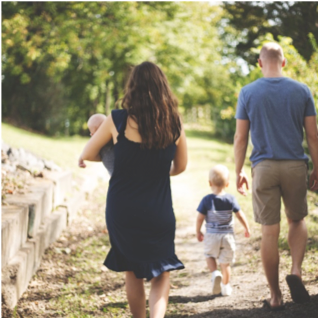
\includegraphics[width=0.70\textwidth]{img/personas/mandick}
\end{minipage}

Mit der vierköpfigen Familie Mandick kommt eine eher spontane Persona in die Auswahl.
Die beiden Eltern können aufgrund ihrer beiden jungen Kinder kaum verlässlich vorausplanen, weshalb sie öfters, jedoch eher unregelmäßig, mit der ganzen Familie ins Kino gehen.
Von der technischen Erfahrung her liegt die Familie zwar etwas hinter den bisher beschriebenen Personas, jedoch nutzen auch sie im Alltag Smartphone, PC und Fernseher, weshalb zumindest grundlegende Kenntnisse durchaus vorhanden sind.

% -------------------------------------------------------
% Oma Gertrud
% -------------------------------------------------------
\newpage
\cvsect{Oma Gertrud}
\begin{minipage}[t]{0.5\textwidth} 	\vspace{0.0\baselineskip} % Required for vertically aligning minipages
	\begin{entrylist}
		\entry
		{Name:}
		{Oma Gertrud}
		\entry
		{Alter:}
		{73}
		\entry
		{Tätigkeit:}
		{Rentnerin}
	\end{entrylist}
	\begin{barchart}{5.0}\hspace{-1.5mm}
		\baritem{Skills}{1}
	\end{barchart}
\end{minipage}
\hfil
\begin{minipage}[t]{0.4\textwidth} 	\vspace{0.0\baselineskip} % Required for vertically aligning minipages
	\flushright
	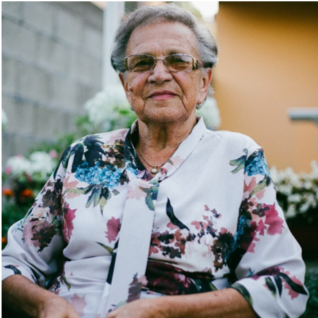
\includegraphics[width=0.70\textwidth]{img/personas/oma_gertrud}
\end{minipage}

Während bei den vorigen Personas von einer gewissen Technikaffinität ausgegangen wurde, repräsentiert Oma Gertrud die Art von Nutzern, die im Alltag kaum Kontakt mit Smartphone, PC oder Tablet haben.
Oma Gertrud passt aufgrund ihres hohen Alters genau in diese spezifische, eher seltene Nutzergruppe.
Durch ihre eher traditionellen Lebensweise konnte sie bisher kaum Erfahrung im Umgang mit moderner Technologie sammeln, was viele für den Durchschnittsnutzer offensichtliche Operationen für sie schwer verständlich macht.
Diese Nutzer sollen trotz ihrer geringen Erfahrung in der Lage sein, zumindest die Basisfunktionen der Website (Ticketreservierung oder -kauf) problemlos durchführen zu können.